% Copyright (c) 2014,2016,2018 Casper Ti. Vector
% Public domain.

\chapter{云环境中的异构硬件为人工智能带来的机遇与挑战}
% \pkuthssffaq % 中文测试文字。
随着硬件技术的不断发展,云环境中支持机器学习任务的硬件也从单一的CPU变成了包含CPU、GPU、FPGA\parencite{putnam2016a}、TPU\parencite{cass2019taking}以及SGX\parencite{costan2016intel}等安全硬件的异构资源。利用这些异构资源,可以给机器学习任务带来一定增益。例如GPU,TPU和FPGA等硬件的SIMD计算模式天然适合ML这种迭代式、大批量的负载,从而可以大大加速ML训练。而诸如SGX等硬件由让机器学习安全有了从硬件层面得到解决的可能性。

而异构硬件为ML任务带来机遇的同时,也带来了一定的挑战。例如,在公有云共享资源池的背景下,如GPU和FPGA等新兴加速硬件没有成熟和系统的虚拟化方案,用户的使用这些硬件的模式仍然以独占为主。即便是共享,也没有成熟的隔离机制保证性能以及用户之间不会相互干扰。再比如,SGX加持的安全计算环境中,可信内存的大小十分有限,如何在有限的资源下支持可信的模型部署甚至模型训练,是亟待解决的问题。

本章将以加速型硬件GPU和安全型硬件SGX为主,介绍云环境中异构硬件为机器学习任务带来的机遇与挑战。

\section{云环境中机器学习作业对GPU的利用}

本节将先对GPU的现状做简要介绍,包括现代GPU的架构以及常见的GPU API和编程模型。然后,本章将从两个角度展开当前学术界针对ML任务对GPU的利用的研究:1)One Job on Multi GPUs。即一个ML任务需要多个GPU设备。这种情况一般出现在大型模型的分布式训练中。在一个大规模GPU集群中,不同的训练任务对GPU数量的需要可能不一样,如何对这些任务进行调度,使系统的资源利用率最高,同时保证训练任务的性能,是学术界研究的重点问题;2)Multi Jobs on one GPU。即在同一个GPU设备运行多个ML任务。这种情况在资源短缺或多租户的场景下较为常见。

\subsection{GPU简介}

\subsubsection{GPU架构}
GPU,即Graphics Processing Unit,采用了与传统的多核处理器完全不同的架构\parencite{hong2017gpu}。GPU的设计围绕和让吞吐率最大化这一原则,提供了上千个简单的计算核心和高带宽内存。这样的实际使得GPU能够使一个应用程序拥有很高的并行度,从而使程序的吞吐率最大化。理想情况下,对于一个GPU应用程序,其包含的若干线程应该分别对应其数据空间的不同位置,而彼此之间由没有因果关联,从而可以并发地执行。与之相反,传统的处理器是为了能更快地执行线性的代码段而优化的。因此其单个核心的复杂度非常高,且单个处理器中的核心数量相对较少。且传统的处理器一般会使用复杂的控制逻辑和较大的本地缓存以处理传统程序中常见的条件分支、上下文切换以及较差的数据本地行。

\begin{figure}[h]
    \centerline{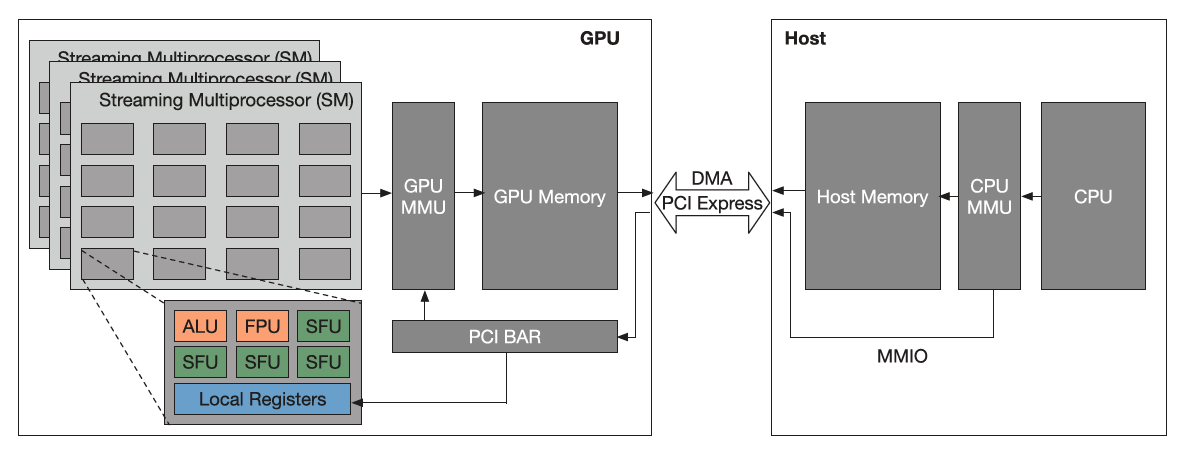
\includegraphics[width=\textwidth]{figures/gpu-arch.png}}
    \caption{GPU系统架构。}
    \label{gpu_arch}
\end{figure}

图~\ref{gpu_arch}展示了一个典型的GPU系统的架构。图中的GPU部分是根据Fermi架构的Nvidia GPU,但是现代的GPU(例如新一代的Nvida GPU和AMD GPU)也遵循类似的设计。一个GPU拥有多个流式处理器(streaming multiprocessor,SM),每一个SM拥有32个计算核心。每个SM也拥有L1数据缓存和低延迟共享内存。每个计算核心拥有本地的寄存器、一个整型计算单元(Integer Arithmetic Logic Unit,ALU)、一个浮点计算单元(Floating Point Unit,FPU)以及若干特殊函数单元(Special Function Units,SFU,用来计算特定的函数值,例如正弦函数sine和余弦函数cosine)。GPU的内存管理单元(MMU)为GPU程序提供虚拟地址空间。MMU会根据应用程序的页表,会将一个GPU地址解析为物理地址。

Host通过PCI高速通道(PCIe)与GPU连接。Host上的CPU通过内存输入/输出映射(MMIO)与GPU进行交互。GPU寄存器以及设备内存可以被CPU通过MMIO接口直接获取。此外,量比较大的数据交换可以通过DMA(Direct Memory Access)实现。DMA可以将数据在设备内存和主机内存之间快速传输。

\subsubsection{GPU API和编程模型}
常用的GPU API和编程模型包括OpenGL\parencite{buck2004brook},Direct3D\parencite{blythe2006the},CUDA\parencite{nickolls2008scalable}和OpenCL\parencite{stone2010opencl}等,在游戏开发、图像处理、高性能计算等场景下非常常用。

OpenGL是一个利用GPU硬件加速图形处理的库,通常应用于电子游戏、图像处理以及科学计算中的数据可视化。OpenGL实现了一个硬件无关的API,兼容适配不同的底层硬件。

Direct3D是由Microsoft Windows提供的图形库,通常在一些性能敏感的场景中(例如电子游戏)负责图形渲染工作。Direct3D同样实现了硬件无关的API,并且向用户暴露了能够使用GPU高级特性的API,例如Z-buffering,W-buffering等。

CUDA是由Nvidia提供了专为Nvidia GPU适配的并行加速库。CUDA允许开发者在GPU上利用高并行的特点开发特定的程序,这种情形下的GPU被称为GPGPU(General Purpose GPU)。CUDA API是与编程语言高度绑定的,例如C和C++。当前流行的机器学习框架,例如Tensorflow和Pytorch,在存在GPU设备的环境中,都支持利用CUDA对其模型训练进行加速。

OpenCL也是一个并行加速库,其基础功能和CUDA类似,最大的区别在于OpenCL可以被应用于非Nvidia的GPU。

\subsection{One Job on Multi GPUs: 机器学习集群中的GPU调度算法}
%SC 17 Topology-aware
%NSDI 19 Tiresias
%OSDI 20 HiveD
事实上,传统集群中的调度算法例如FCFS(First-come,first-served),Round-robin,Priority-based,Fair queuing\parencite{demers1989analysis}等经典算法,在GPU集群中仍然适用。这些算法简单地将GPU看作一种新的资源单位,并将提交到该集群中的作业调度在其上。

随着深度学习的兴起和快速发展,在计算机视觉、自然语言处理等领域使用的模型参数越来越多,规模越来越大。而对于大规模的深度学习模型,分布式训练+GPU硬件加持几乎成为了标配。分布式训练的场景中,GPU之间的数据传输时有发生。然而在一个多GPU的集群环境中,位于整个系统拓扑结构不同位置的GPU之间的数据传输速度是有很大差异的。因此,仅使用传统的的调度算法,而不考虑GPU设备之间的拓扑结构,很可能会造成糟糕的调度结果,从而严重影响作业性能。

\begin{figure}[h]
    \centerline{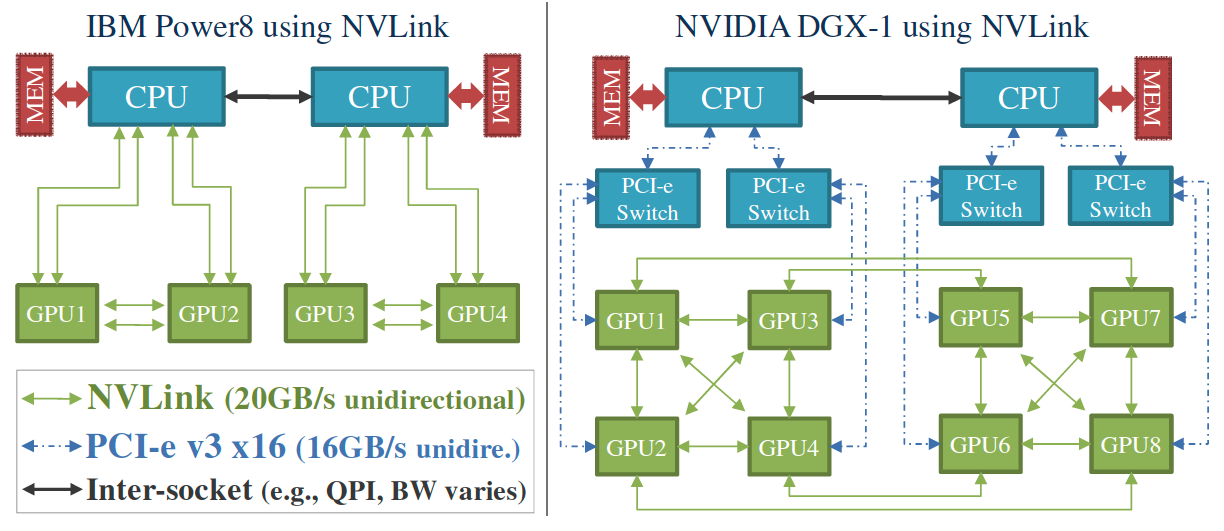
\includegraphics[width=\textwidth]{figures/gpu-topology.png}}
    \caption{GPU拓扑结构示例。}
    \label{gpu_topology}
\end{figure}

图~\ref{gpu_topology}展示了两个GPU服务器中GPU的和其它硬件之间的拓扑结构图。左图为IBM的Power8服务器,有两个CPU和四个GPU。右图嵬NVIDIA和DGX-1服务器,有两个CPU、四个PCI-e桥接器和8个GPU。绿色的线、蓝色的线和黑色的线分别代表NVLink\parencite{foley2017ultra}、PCI-e和Intel的QPI三种连接方式,数据传输速度由快到慢。位于同一个CPU socket下的两个GPU(例如左图中GPU1和GPU2)之间的数据传输可以通过NVLink进行,是最快的。位于不同CPU上的GPU,只能通过PCI-e通道和QPI通道进行通信(例如左图中的GPU1和GPU3、右图中的GPU1和CPU)。而如果位于两台不同服务器上的GPU之间需要通信,则除了需要经过上述数据通路之外,还要经过网络传输,即时是万兆网(10Gbps),也要比上述传输方式慢约一个数量级。

\begin{figure}[h]
    \centerline{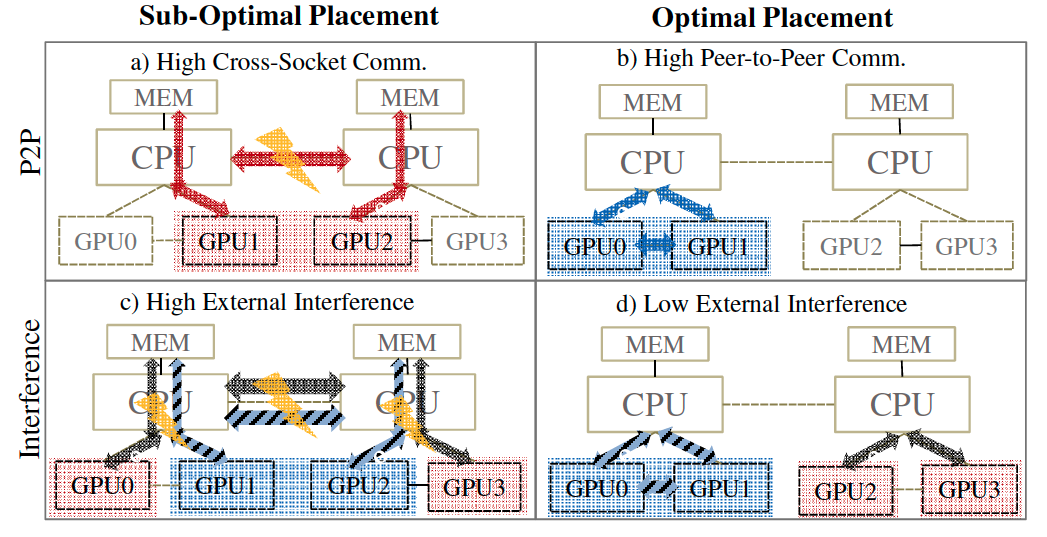
\includegraphics[width=\textwidth]{figures/gpu-top-sub-opt.png}}
    \caption{GPU调度示例。}
    \label{gpu_top_sub_opt}
\end{figure}

因此,在GPU集群中调度分布式ML训练任务时,需要充分考虑GPU之间的拓扑结构,否则可能会造成严重的性能损失。图~\ref{gpu_top_sub_opt}展示了GPU调度的两个例子和与其对应的四种调度方案。上面的两张图对应了P2P(即两个GPU之间需要互相通信)的场景中的两种调度方案,显然右边的方案是更优的方案,因为分配到的两个GPU位于同一个CPU socket上,于左边相比其数据通路具有更高的传输速率。下面的两张图对应了不当分配可能造成的性能干扰。显然,右边的分配方式也是更优的方式,因为左边的分配方式造成了两个Job在数据传输时共用同一条数据通路从而造成竞争,使性能降低。

M. Amaral等人\parencite{amaral2017topology}在2017年提出了一种云环境下基于GPU拓扑结构的调度方法。其将ML任务和集群都抽象成图的形式。在ML的任务图中,图的节点为GPU,节点之间的边代表两个GPU之间存在数据交流。任务图中的边没有权重。在集群的图中,图的节点为CPU,GPU,PCI-e桥接器,CPU socket或者网络交换机。不同节点之间的连线代表这两个节点之间可以相互通信,连线的权重代表通信速度,数值与越小通信速度越快。图~\ref{gpu_graph}表示了图~\ref{gpu_topology}所对应的拓扑结构图。

\begin{figure}[h]
    \centerline{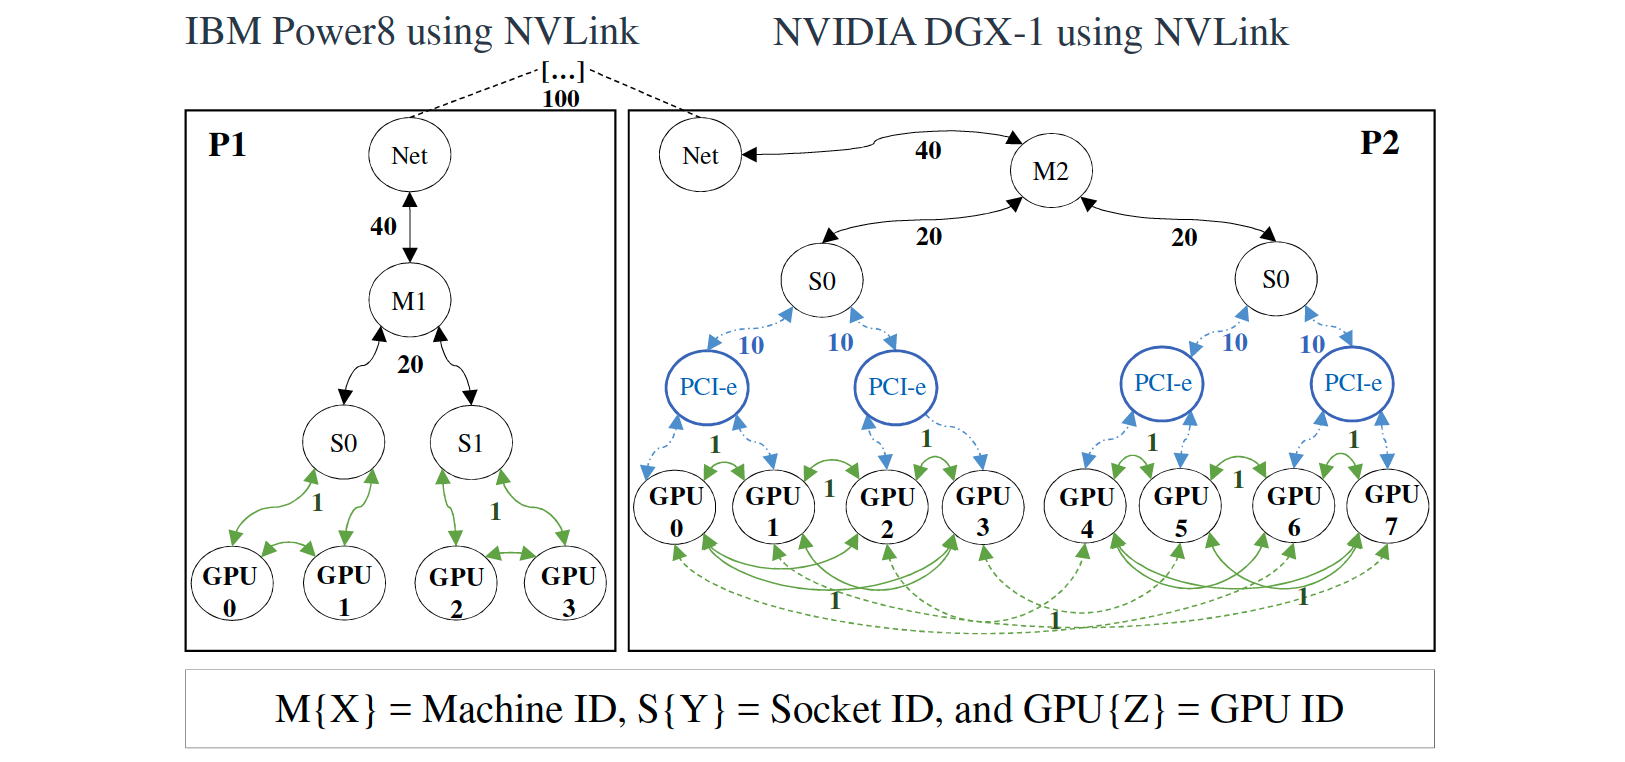
\includegraphics[width=\textwidth]{figures/gpu-graph.png}}
    \caption{GPU拓扑结构图。}
    \label{gpu_graph}
\end{figure}

M. Amaral等人通过对两个图进行匹配并最小化公式~\ref{eq_top_min}中的目标来实现GPU的调度,其中$\alpha^{cc}+\alpha^b+\alpha^d=1$,$t$、$I$和$\omega$分别代表GPU之间的通信代价、来自外部的资源干扰和资源碎片化程度,分子代表实际的值,分母代表最坏情况下的值。该公式旨在综合考虑减小GPU之间的通信代价、降低不同任务之间的干扰以及使整个系统的碎片化尽可能降低,使整个集群处于一个相对最佳的状态。

\begin{equation}\label{eq_top_min}
    MIN\ \alpha^{cc}\frac{t^{cc}}{t_w}+\alpha^b\frac{I^b}{I_w}+\alpha^d\frac{\omega^d}{\omega^w}
\end{equation}

\begin{figure}[h]
    \centerline{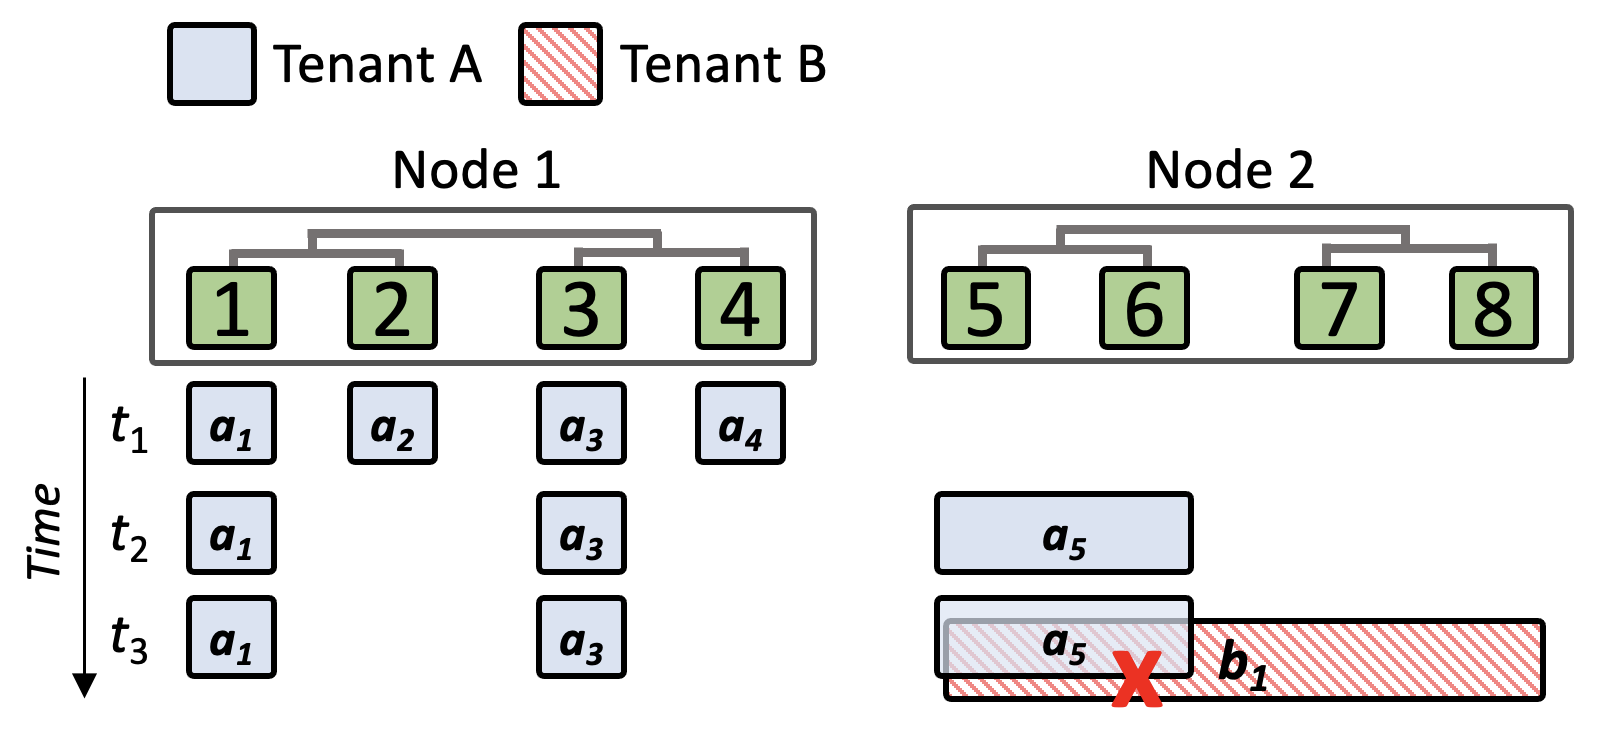
\includegraphics[width=\textwidth]{figures/hived-pendding.png}}
    \caption{GPU集群中的调度异常:一个任务被阻塞。}
    \label{hived_pending}
\end{figure}

M. Amaral等人的工作综合考虑了多项指标,以使得集群达到一个最优状态。在这样的集群中,所有的任务都被视作拥有同样的优先级。因此,可能存在集群中常见的长尾问题。图~\ref{hived_pending}就描述了这样一个场景。租户A和租户B都需要使用GPU,然而由于调度问题,虽然集群中还剩余4个GPU,却无法分配给B。这种情况被称之为调度过程中的异常(anomaly)。

H. Zhao等人在2020年提出了HiveD\parencite{zhao2020hived},使用Virtual Private Cluster的概念和伙伴算法(即Buddy Cell算法)来解决调度中的异常。HiveD中将任务分为两类:高优先级的需要保证资源的任务和低优先级的尽可能用“机会性资源”来提升集群资源利用率的任务。其使用的伙伴算法在Linux内核中的内存管理模块中也是常用的算法。图~\ref{hived_diff_view}表达了HiveD中两类任务中不同的资源视角。HiveD中将GPU按照连接方式划分为不同级别的Cell,如图中单个GPU称为Level 1的Cell,位于同一个CPU socket上的两个GPU称为Level 2的Cell,位于同一CPU下的四个GPU称为Level 3的Cell,位于同一台服务器下的八个GPU称为Level 4的Cell,位于同一机架上的不同服务器上的GPU集合称为Level 5的Cell。HiveD假设任务对于GPU需求都是与某一个Level的Cell中的GPU数量匹配的,其基本算法思路如下:当有一个任务需要一个Level k的Cell时,先查看系统中有无现有空载的Level k的Cell,如果没有则将一个Level k+1的Cell分裂为两个Level k的Cell,如果再没有则继续向上一层Cell请求分裂,直到存在空载的Cell为止。同时,如图~\ref{hived_diff_view}所示,高优先级和低优先级的任务视角中,资源的使用情况是不同的。如果一个Cell被高优先级的任务占用,则在低优先级任务的视角中,这个Cell被标记为“已使用”,不能被抢占。反之,低优先级任务占用的Cell在高优先级任务的视角中被标记为dirty,在必要的情况下可以抢占其使用。

\begin{figure}[h]
    \centerline{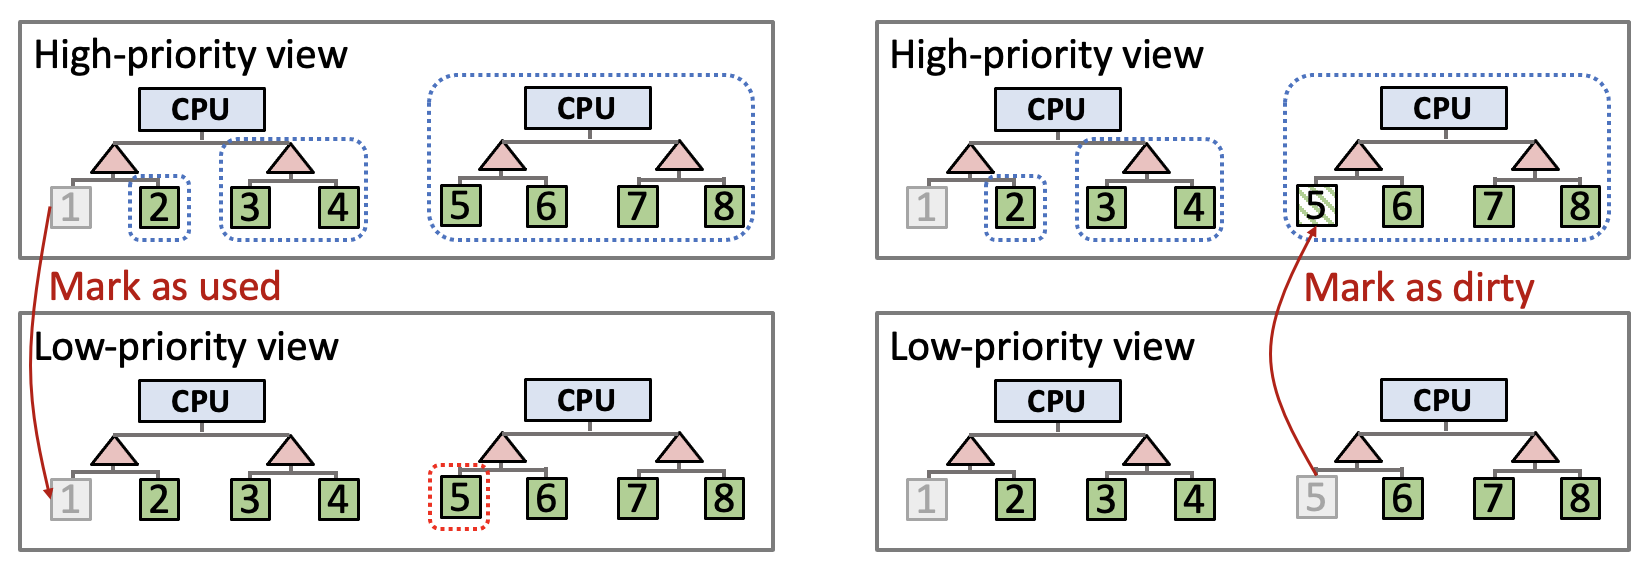
\includegraphics[width=\textwidth]{figures/hived-diff-view.png}}
    \caption{HiveD中的两种视角。}
    \label{hived_diff_view}
\end{figure}

总体而言,与传统的集群资源调度其类似,以GPU设备为最小调度单位的系统调度器中,首要的目标是保证集群的吞吐率,即单位时间内处理任务的数量。近年的做法都是基于GPU之间的互联情况对GPU设备(组)进行分类,进而使用各种算法使任务的需求与系统当前的状态匹配,达到降低任务运行时间、提升系统吞吐率的目标。在此基础上,在一些碎片化的资源上部署一些低优先级的作业,可以进一步提升系统的资源利用率。

\subsection{Multi Jobs on one GPU: 机器学习集群中的GPU共享机制}
%OSDI 18 Gandiva
%MLSys 20 Salus
除了以单个GPU为单位,在真实的业务场景中也存在多个任务共享同一个GPU的需求。该需求出现于云计算刚刚兴起的早期,即如何对GPU进行虚拟化。常用的应将资源例如CPU,网络和存储等都有非常成熟的虚拟化方案。以CPU为例,常见的虚拟化一般可以分为虚拟机和容器两大类。虚拟机有着比云计算更悠久的历史。IBM 公司在1970年阐述了其最原始的虚拟机系统设计\parencite{goldberg1974survey}。在1972 年,虚拟机第一次在 IBM 公司的大型机上出现。通过IBM VM370系统能够将一台大型机分为可独立运行操作系统的多台虚拟机。在计算虚拟化技术中,原本的物理计算机被称为宿主机(Host),运行在宿主机之上的虚拟机被称为客户机(Guest)。虚拟机技术的核心是VMM(虚拟机监控器 Virtual Machine Monitor 或者虚拟机管理器 Virtual Machine Manager),也被称为Hypervisor\parencite{barham2003xen}。容器是进些年来更受关注的轻量级虚拟化技术。与虚拟机技术不同,容器并不对 CPU 指令以及硬件设备进行虚拟化,它是一种操作系统级的虚拟化技术。容器通过操作系统内核提供的功能,来实现不同用户进程的资源隔离与访问隔离,形成一个个独立的运行时环境,即“容器”。

云计算的兴起离不开虚拟化的发展。当前,主流的云厂商例如AWS,Google Cloud等,都同时提供了虚拟机服务和容器服务。这些服务基于对计算资源(主要是CPU)、网络资源(带宽、虚拟网络)和存储资源(虚拟云盘)的虚拟化,支持用户在虚拟计算环境中独立且互不干扰地运行各种负载。然而GPU作为现今一种重要的计算资源,却始终没有一种统一的、完善的虚拟化方案应用于公有云环境,而是在不同的业务场景中存在不同的虚拟化方案。

根据实现方式的不同,当前GPU的虚拟化大致可以分为三类\parencite{hong2017gpu}:

\textbf{1. API转发。}这种方式在GPU架构的上层对GPU进行虚拟化。由于GPU的厂商一般不会开源GPU的驱动源码,因此在驱动层对GPU进行虚拟化是非常困难的。基于API转发的虚拟化实现方式类似于远程过程调用(Remote Procedure Call,RPC),即在虚拟机OS中实现一个agent,该agent会截获应用程序所有对GPU的调用,并将相关调用转发到宿主机上的GPU设备上进行实际的执行,执行完毕后再返回给虚拟机OS中的应用程序。

\textbf{2. 半/全虚拟化。}这种方式在驱动层对GPU进行虚拟化(一般由厂商来实现),一般会定制一个专门的driver安装在虚拟机OS中。与API转发相比,这种方式由driver直接调用宿主机的driver API,不需要你agent的转发,从而缩短了调用链,使其性能更优。

\textbf{3. 基于硬件的虚拟化。}这种方式也称为pass-through(译作直连),即赋予虚拟机直接访问宿主机设备的能力。这种方式产生的额外开销是最小的,但是一般而言隔离型比较差。

上述三种方式中,API转发是学术界的工作最为常用的方法,无论是在基于虚拟机的环境中,还是在基于容器的轻量级虚拟化环境中。图~\ref{api_remoting}描述了虚拟机环境中基于API转发的GPU虚拟化的工作流程。

\begin{figure}[h]
    \centerline{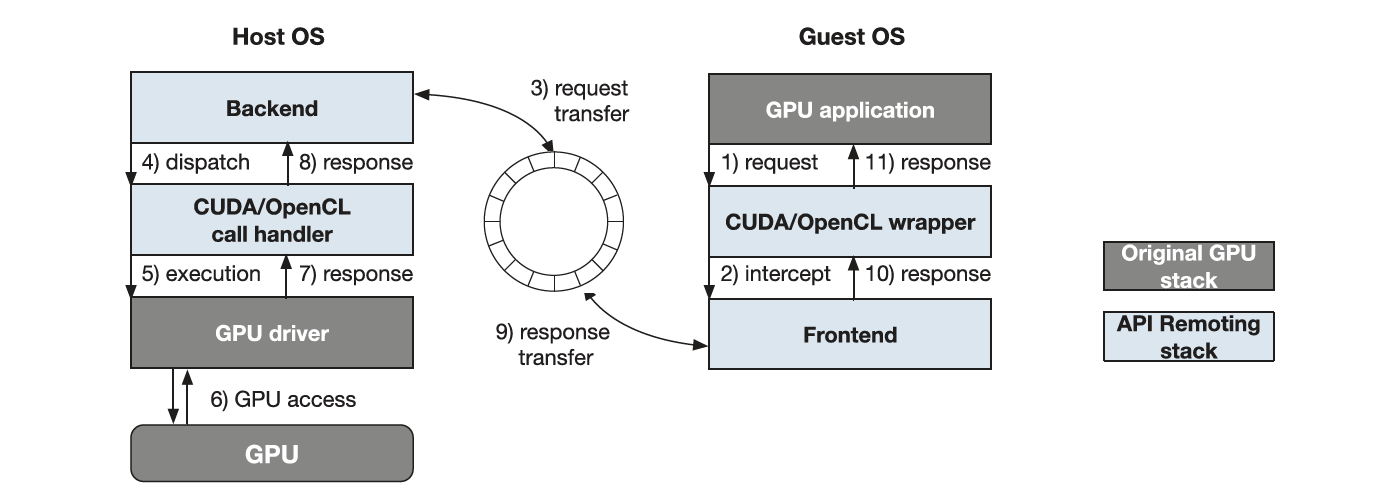
\includegraphics[width=\textwidth]{figures/api-remoting.png}}
    \caption{基于API转发的GPU虚拟化。}
    \label{api_remoting}
\end{figure}

\begin{figure}[h]
    \centerline{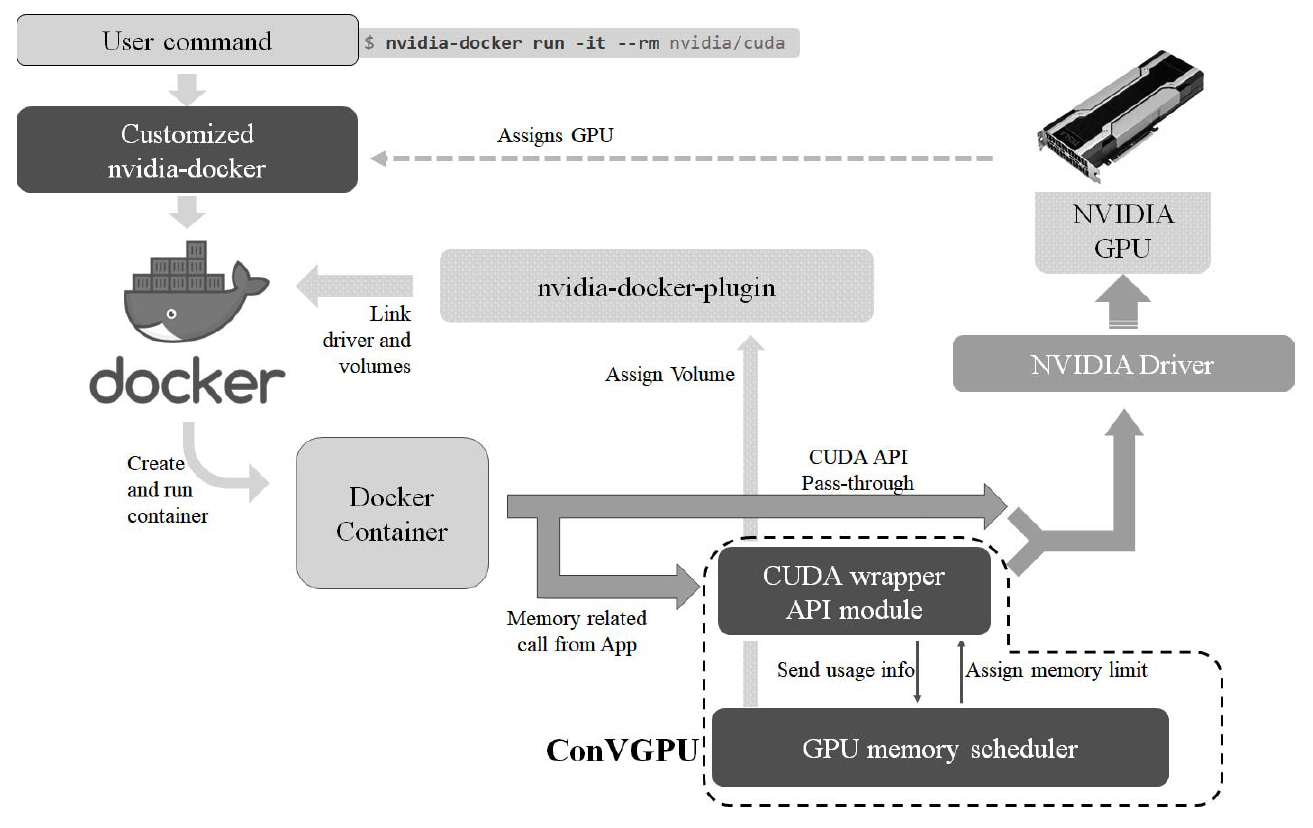
\includegraphics[width=\textwidth]{figures/convgpu.png}}
    \caption{ConVGPU架构。}
    \label{convgpu_arch}
\end{figure}

在容器环境中基于API转发的方式和上图类似。D. Kang等人在2017年提出了ConVGPU\parencite{kang2017convgpu},通过在docker容器中安插一个CUDA wrapper来对一些与GPU显存相关的API(例如cudamelloc,cudafree等)进行截获,并实现了一个管理全局显存分配的调度模块。如图~\ref{convgpu_arch},ConVGPU实际上是以一个中间件的形式存在于容器环境中的。在正常的API调用路径下,插入一个显存管理的组件,在软件层面实现了GPU显存的共享和一定程度上的隔离。

而更多的GPU共享的解决方案是与具体的应用场景高度绑定的,尤其是在运行机器学习任务的集群中。W. Xiao等人在2018年提出了Gandiva\parencite{xiao2018gandiva},主要面向深度学习集群中基于GPU的模型训练任务进行调度。有别于传统的suspend/resume机制,Gandiva使用grow/shrink机制。图~\ref{gandiva_grow_shrink}表现了Gandiva的grow-shrink机制。Gandiva中主要存在如下三种动作:1)grow。即当前如果存在空闲的资源,Gandiva会让存在空闲资源的节点上的某些任务占用的资源拓展到空闲资源上,以提升系统的资源利用率和模型的训练速度(如图~\ref{gandiva_grow_shrink}中的Gandiva:(3) Grow-shrink)。2)shrink。当系统中有新的训练任务到达时,Gandiva一般不会将一个任务直接shutdown,而是将其所占用的资源进行裁剪,腾出新的资源以供新的任务所用(如图~\ref{gandiva_grow_shrink}中的Gandiva:(3) Grow-shrink)。3)migration。当系统其它节点中存在空闲资源时,Gandiva会将一个非独占的任务迁移到该空闲资源上(如图~\ref{gandiva_grow_shrink}中的Gandiva:(2) Migration)。值得注意的是,Gandiva在实验中发现,深度学习任务的显存占用一般呈周期性涨落的趋势,其峰值显存占用率和谷值显存占用率差距非常大。因此其在迁移任务时会根据任务占用显存的变化趋势,在任务占用显存最小的时候对任务进行迁移,以降低迁移产生的额外开销。

\begin{figure}[h]
    \centerline{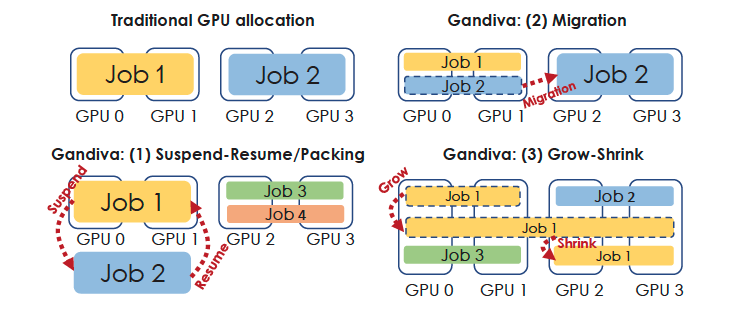
\includegraphics[width=\textwidth]{figures/gandiva-grow-shrink.png}}
    \caption{Gandiva grow/shrink机制。}
    \label{gandiva_grow_shrink}
\end{figure}

事实上,Gandiva中所提到的深度学习任务显存占用的周期性涨落趋势,也可以用来实现更细粒度的GPU共享。P. Yu等人在2020年提出了Salus\parencite{yu2020salus},使用快速任务切换和显存贡献实现GPU的共享。Salus将显存分成多个Lane,一个Lane中可以存在一个或者多个深度学习模型训练任务。由于深度学习模型训练任务都是周期性迭代的过程,Salus调度的最小单位是任务的一个周期(在模型训练中通常体现为一个batch)。图~\ref{salus_arch_sche}展示了Salus的架构和一个调度示例。Salus为常用的ML框架如Tensorflow和Pytorch定制了相应的适配器。对于用户的模型训练程序的每一次迭代周期,都会以一个session的形式提交到Salus的session管理器。Salus根据提交的session的显存变化曲线,将session调度到合适的Lane中。然后调度器根据系统当前显存分配的状况,调度相应的Lane在GPU上执行。右图中即为一个例子,Job 1 和Job 2在显存变化曲线上存在明显的互补性,使得Job 2的波峰恰好可以将Job 1的波谷填满,因此Salus调度其在同一个Lane上执行。

\begin{figure}[h]
    \centerline{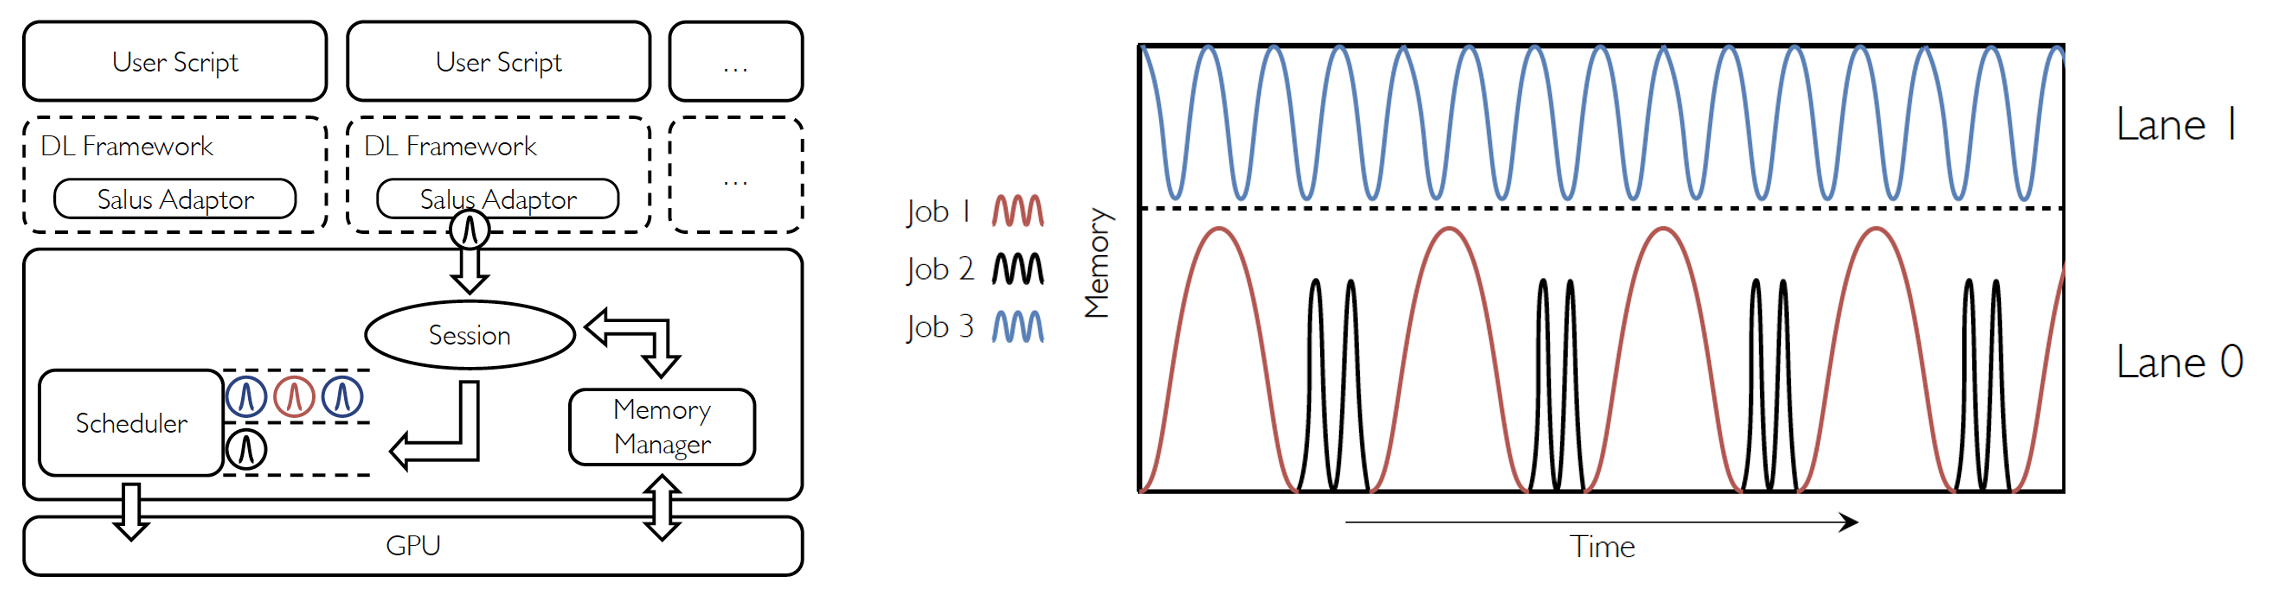
\includegraphics[width=\textwidth]{figures/salus-arch-sche.png}}
    \caption{Salus架构与调度示例。}
    \label{salus_arch_sche}
\end{figure}

除了模型训练中对GPU的共享之外,近年来也有学者开始研究模型部署阶段对GPU共享。D. Mendoza等人\parencite{10.1145/3437984.3458837}在2021年提出了一种干扰可感知的模型部署调度。该调度方法充分关注模型推断期间的系统指标,例如CPU利用率的变化曲线,设计模型学习不同的ML任务共同部署时对性能的干扰,进而将该信息应用到调度中,以提升共同部署的模型的推断效率。

\section{云环境中机器学习作业对SGX的利用}
能够安全可信地使用由第三方云厂商提供的计算服务是云消费者的重要需求。尤其是当前人工智能技术盛行,很多个人开发者、研究团队和中小型公司都有利用公有云算力训练机器学习模型的需求。但是这些用户需要将具有一定私密性的数据上传到云厂商,这在一定程度上是具有潜在的安全性风险的。因此用户需要以一种安全的方式对云资源进行利用。当前,能够满足这一需求的主流解决方案包括同态加密(Homomorphic Encryption)\parencite{shacham2013compact}和可信执行环境(Trusted Execution Environment)\parencite{seibel2017trusted}。同态加密是一种密码学技术,可以对加密后的密文直接进行计算,并且计算结果解密后与明文计算的结果相一致。2009年斯坦福大学的C. Gentry首次提出了通用的同时支持加法同态和乘法同态的全同态加密方法\parencite{gentry2009fully},在理论上证明了云计算资源安全使用的可能。用户可以将数据加密后在云端进行计算,然后将结果传输回本地进行解密,这样可以同时做到既依赖了云端的强大算力又保证了数据安全性。但由于该方案引入了巨大的计算开销,出于性能原因至今仍然没有得到广泛的使用。

可信执行环境是一种基于硬件的解决方案,其本质上相当于为用户提供了一种安全的沙箱环境。用户可以在可信执行环境中进行计算,并且能够得到机密性和完整性的保障,而包括Hypervisor、操作系统、主机上可信执行环境以外的其他应用都没有权限读写可信执行环境中的数据,从而保证了用户使用云计算资源的安全性。代表性的可信执行环境实现包括Intel的SGX技术和ARM的TrustZone\parencite{azab2014hypervision}技术。相比于全同态加密,这些技术有着更高的计算效率,近年来在云计算环境下有着强隐私保护需求的许多场景里得到了实际应用。因此,本节主要着眼于可信执行环境这种云计算资源在机器学习场景下的安全性利用方案,以Intel SGX技术为重点,对相关技术进行调研。

\subsection{SGX技术简介}
可信执行环境是解决服务使用者与供应者之间信任问题的一种流行方案。在服务器端,英特尔软件保护扩展(Intel Software Guard Extensions,SGX)是目前最主流且被使用最多的可信执行环境技术,用于保护运行在不受信任平台上程序的机密性(Confidentiality)和完整性(Integrity),于2015年在Intel Skylake系列的CPU\parencite{costan2016intel}中首次被推出。图~\ref{sgx_arch}概述了SGX的简单特性。SGX提供了被称为飞地(Enclave)的硬件安全沙箱,用于托管用户代码和数据,防止其被飞地外不受信任的特权进程(例如Hypervisor 和操作系统)窃取或篡改。本章提出的解决方案基于SGX设计和实现。

\begin{figure}[h]
    \centerline{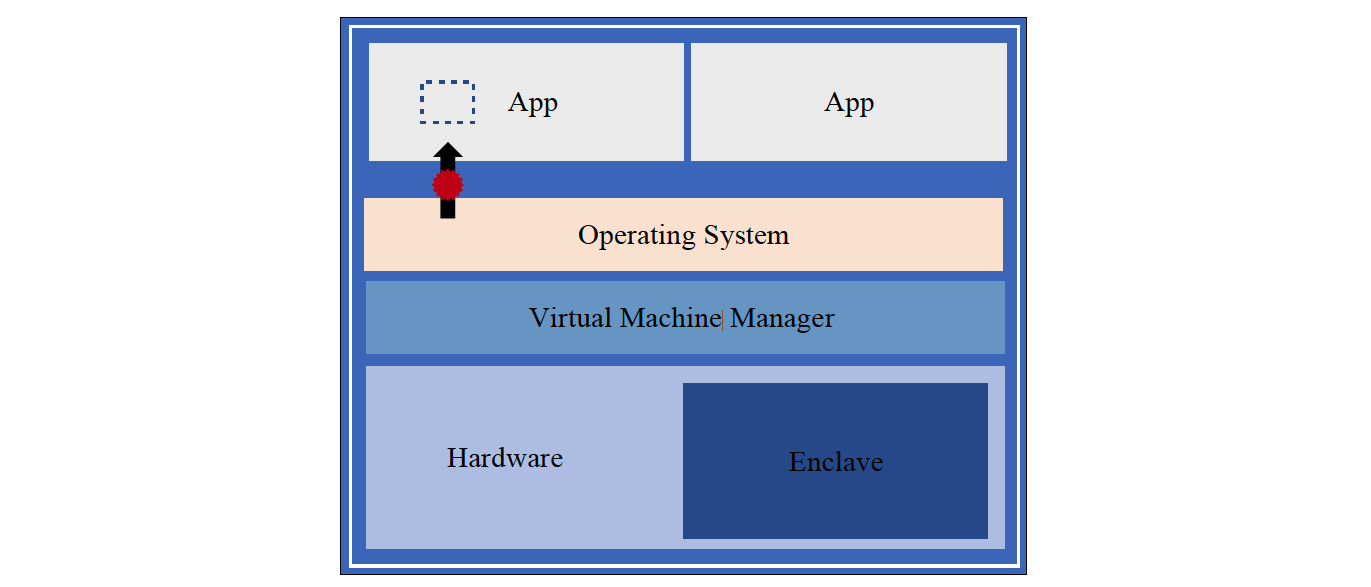
\includegraphics[width=\textwidth]{figures/sgx-arch.png}}
    \caption{SGX架构图。}
    \label{sgx_arch}
\end{figure}

截至2021年3月,SGX包括两个主要版本,最初的版本通常被称为SGX 1.0,另一个版本具有增强的特性,如飞地动态内存管理,被称为SGX 2.0。由于SGX 2.0仅在有限的CPU 系列上支持,因此本文只讨论SGX 1.0,其已经包含了SGX核心的安全特性。SGX技术通过一组CPU 指令扩展和专用硬件架构来构建所谓的飞地。飞地里的代码和数据都运行在特殊的加密内存里,只有飞地里的程序运行在CPU 里时才会对相应的代码和数据进行解密。因此,即使攻击者有机会接触到硬件,通过窥探内存(Hardware Snoop)的方式也只能看到加密后的信息。在一个飞地进行初始化之前,代码和数据保存在主机的非可信区域。同时,SGX也无法保障飞地以外数据的安全性。因此,为了保护秘密,在使用SGX时,数据应该在飞地外进行加密,然后传输到飞地内解密后进行计算。

\textbf{认证(Attestation)}:SGX提供了认证机制,其功能是让用户可以验证一段已知的程序确实是运行在一台支持SGX功能的计算机的飞地里的。认证又包括本地认证(Local Attestation)和远程认证(Remote Attestation)。本地认证使得一个飞地可以向运行在同一平台上的另一个飞地证明自己的身份。远程认证使得一个飞地可以向远程第三方实体证明自己的身份。SGX提供了飞地度量值(即MRENCLAVE和MRSIGNER两个值)用来在认证过程中表明飞地的身份并验证飞地的完整性。

\textbf{密封(Sealing)}:在飞地中运行的代码和数据是易失性的。密封是SGX 提供的一种机制,用于将数据保存到持久化的非可信存储中,例如硬盘。在密封过程中,应用使基于可信执行环境的可信应用快速构建与支撑机制用密封密钥(Sealing Key)在飞地中加密数据。密封密钥只能由该应用的飞地程序获得,并且是从根密封密钥(Root Sealing Key)衍生而来的。根密封密钥则是硬件编码在CPU中,并且每一个支持SGX的CPU的根密封密钥都是互不相同的,这就决定了某一飞地在某台机器上密封的数据只能在该台机器上进行解密。

\textbf{飞地页面缓存(Enclave Page Cache,EPC)}:飞地所驻留的特殊加密内存区域被称为EPC。EPC由专用硬件加密,禁止所有来自非飞地内存的访问。EPC以4KB的粒度划分为页面进行内存分配。飞地在初始化时申请它需要的所有EPC空间,并且在分配之后不能动态修改。EPC的总大小非常有限,在一台计算机上,SGX飞地应用程序可以使用的EPC的大小是128MB。在这其中,只有约93.5MB的大小可供用户程序和数据使用,剩余空间预留用来存储SGX相关的元数据。在当前的大数据时代,EPC的空间过于稀少,并且单机上的EPC会被所有的SGX程序分享,这就导致每一个飞地实际可用的EPC空间就更小了。在服务器市场主流的Linux操作系统上,SGX驱动支持通过页交换技术来实现EPC超配,每个飞地实际可以申请超过128MB的内存使用。当EPC中没有空闲页分配给飞地使用时,SGX驱动程序会基于缓存替换算法将EPC中的某些页面加密后放置到非加密的常规内存DRAM上去。当这些换出的页面在重新被需要使用时又会被换入到EPC 中。因为换入换出页面时涉及到完整性校验等高计算开销的过程,因此会导致应用程序性能的显著降低。先前的工作表明,这种开销平均会使系统性能降低5倍\parencite{taassori2018vault}。由于EPC很小,并且由运行在一台机器上的所有飞地竞争,因此可能会频繁地触发页交换。

\textbf{SGX应用程序开发}:当前主要有两种方式来开发面向SGX的应用程序。第一种是基于功能划分的方式。使用这种方式来开发程序通常需要将整个应用设计为可信与非可信两个部分。敏感数据由运行在飞地内的可信程序处理,其他功能由飞地外的非可信程序完成。使用Intel原生SGX软件开发工具或如一类的开源框架来编写软件是这类开发方式的典型代表。这类方式可以更有效地利用EPC资源,但需要付出较大的努力对传统非SGX环境下的留存应用进行重构。第二种方式是使用库操作系统(LibraryOS,LibOS)\parencite{engler1995exokernel}来进行开发。库操作系统通过实现应用所需的系统调用来支持在飞地内运行整个程序。这种方式为留存应用提供了更好的兼容性,对开发人员更加友好。目前主流的面向SGX环境设计的库操作系统包括Haven\parencite{baumann2015shielding}、Panoply\parencite{shinde2017panoply}、Graphene-SGX\parencite{tsai2017graphene}和Occlum\parencite{shen2020occlum}。

\subsection{基于SGX技术的上层应用}

首先在最基础的容器粒度上,S. Arnautov等人提出了一种基于SGX实现的安全容器SCONE\parencite{arnautov2016scone}。SCONE对SGX进行了进一步的抽象来保护容器中的进程。其为开发者提供了C语言标准库接口来便利地开发基于SGX的应用程序。SCONE的设计中系统调用在可信执行环境之外进行,但通过加密技术保证了可信执行环境之外的数据也是安全的。进一步地,为了降低在可信执行环境中进行线程切换的开销,SCONE将操作系统线程映射为逻辑的应用线程,通过在应用线程间调度操作系统线程来最大化线程在可信执行环境中的运行时间。在易用性上,SCONE兼容Docker,对Docker用户是透明的。在Apache、Redis、NGINX等应用上的测试表明,SCONE可以达到原生应用0.6至1.2倍的吞吐量。

SCONE针对的是单机的容器环境,T. Hunt等人则基于SGX技术设计和实现了面向分布式环境的可信计算中间件Ryoan\parencite{hunt2018ryoan}。Ryoan针对的是无状态、采用面向请求数据模型的应用,其提出了新的执行模型,对不可信代码模块施加限制,并严格执行防止机密泄露的I/O策略。Ryoan可以使得互不信任的多个参与方能够在不受信任的平台上(例如云平台)以分布式的方式进行敏感数据的计算。Hunt等人更进一步地基于Ryoan开发了包括图像处理系统、垃圾邮件过滤器在内的多个真实应用作为研究案例。

\begin{figure}[h]
    \centerline{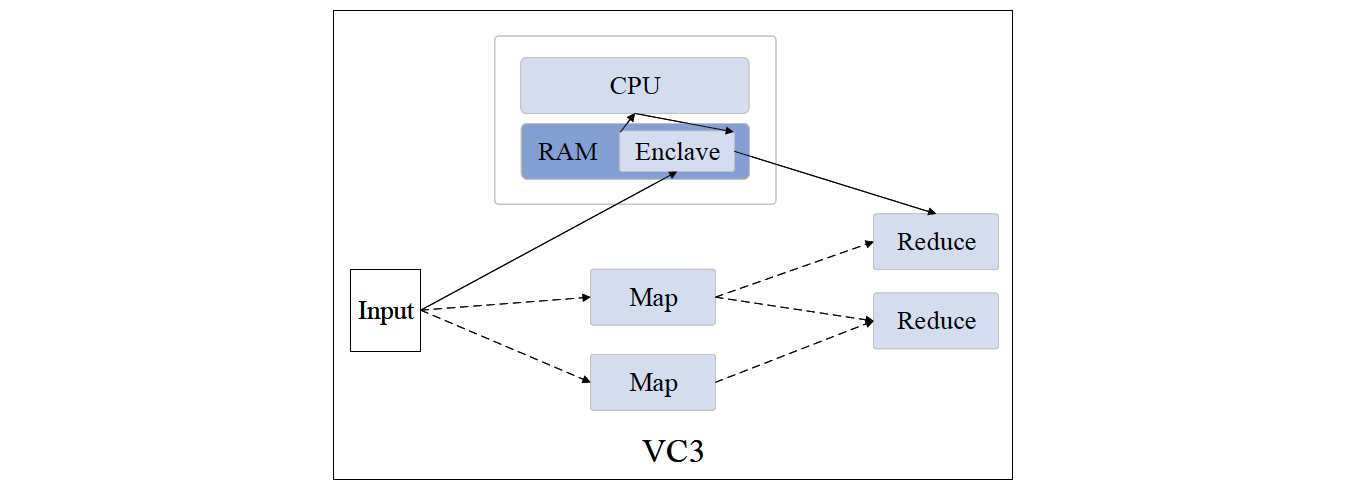
\includegraphics[width=\textwidth]{figures/vc3-arch.png}}
    \caption{VC3架构图。}
    \label{vc3_arch}
\end{figure}

SCONE和Ryoan等都是基于SGX在系统软件这个层次所做的工作,用以帮助开发者更便捷地使用SGX技术。相比之下,VC3\parencite{schuster2015vc3}是更上层的工作,其基于SGX开发了一个可信的分布式数据处理框架,可以运行在未修改的Hadoop之上。图~\ref{vc3_arch}阐述了VC3的设计理念:在VC3中,数据和代码(例如Map和Reduce程序)在可信执行环境之外都是加密的。VC3解决了三方面的问题来使得这个数据处理框架具有实用性:首先,为了实现更轻量级的可信计算基,VC3的设计只将核心的Map和Reduce函数运行在可信执行环境中;其次,可信执行环境只能保证单个Map或Reduce任务的完整性,为此VC3提出了专门的作业执行协议来保证整个分布式计算的完整性;最后,VC3提供了新的编译器支持来防止不安全的内存访问。在通用测试基准数据集上的实验显示,相比于原生Hadoop,实现“写完整性”保护和“读写完整性”保护的VC3仅额外产生了4.5\%和8\%的运行时开销。

\subsection{集群中SGX资源的管理}

可信执行环境技术的实现离不开新的硬件支持。换言之,在支持可信执行环境的计算机上,操作系统管理除传统的CPU、内存、I/O等系统资源以外,还需要管理新型的特殊硬件资源。以Intel SGX为例,其使用了一种特殊的被称为EPC(Enclave Page Cache)的加密内存来运行代码和数据。以EPC为代表的新型硬件的出现给云原生共享集群的管理带来了挑战。共享集群通过让不同的分布式应用共享底层硬件资源来优化系统管理、提升集群资源利用率。“共享”意味着管理系统需要基于虚拟化等技术手段来对资源进行抽象和隔离,防止不同应用程序在共享硬件资源时因竞争而产生相互干扰,导致性能下降甚至是程序崩溃等问题。

对于传统的CPU、内存、I/O等硬件资源,当前的操作系统已具备成熟的机制(如容器)对其进行隔离。共享集群管理系统也依赖于操作系统的这种能力来完成资源分配、变更和调度。但遗憾的是,当前的操作系统虚拟化和隔离可信执行环境所依赖的新型硬件资源的能力还较为有限,这给云原生共享集群在利用这些资源时带来了挑战。以现有的共享集群管理系统为例,YARN尽管提出了容器的概念用以进行资源划分和分配,但那只是一种逻辑的抽象,在实际运行时,YARN并没有将任务封装在LXC、Docker之类的操作系统虚拟化容器中。在早期的版本中,YARN只对内存这单一维度的资源进行限制。当YARN启动一个任务时,同时还会启动一个监控器对任务进程的内存消耗进行监控。当任务进程消耗的内存超过任务申请的内存时,YARN会将该任务终止。而对于如CPU之类的其他资源,尽管用户在提交作业时也会为每个任务指定申请的资源配额,但这些信息仅仅会被用来进行调度决策,YARN不会对这些资源进行限制。因此,一个指定了1个CPU核数的任务在机器较为空闲时可能会使用超过1个CPU核数的资源。随着时间的发展,在后续版本中,YARN引入了cgroups机制,通过cgroups实现了对CPU、I/O等资源的限制。

因为YARN启动任务就是启动进程,如果想在YARN中运行SGX任务,只需在集群节点上安装好SGX驱动程序等相关环境即可。但当前的YARN缺少接收任务使用EPC资源需求的接口,因此YARN在调度时不会考虑SGX作业需要使用多少EPC资源。进一步地,YARN缺乏隔离EPC的能力,因此调度到同一台机器上的两个SGX程序会竞争EPC使用,导致程序性能下降。

与YARN 相比,Kubernetes管理和编排的是以Docker为代表的操作系统虚拟化容器。也就是说,在Kubernetes中,任务进程都是运行在Docker容器里的。对于SGX任务而言,如果想要以Docker的形式运行,需要将主机上的\textit{isgx}设备文件映射到容器里。在Kubernetes里运行SGX任务则更复杂一些,需要使Kubernetes具备管理EPC的能力。

\begin{figure}[h]
    \centerline{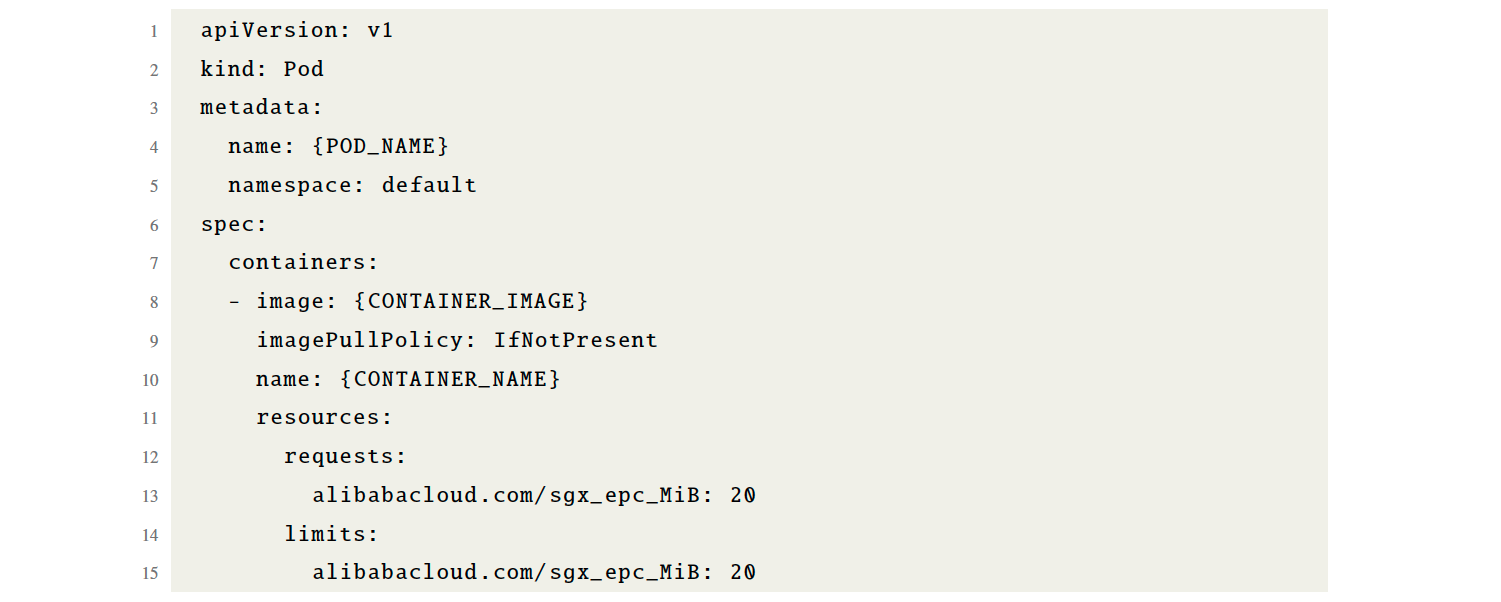
\includegraphics[width=\textwidth]{figures/k8s-yaml.png}}
    \caption{使用SGX设备插件在Kubernetes中提交任务时编写yaml文件。}
    \label{k8s_yaml}
\end{figure}

Kubernetes 提供了一套被称为设备插件(Device Plugin)的机制来接入新型硬件设备,例如SGX、GPU、FPGA等。设备插件提供一个RPC服务接口向kubelet进行注册,发送管理的设备列表。kubelet是Kubernetes运行在每个节点上的代理,它会进一步地将这些硬件资源信息发送到集群主节点上的API服务器中。用户在请求使用这些新型硬件资源时,可以在配置文件yaml中指定这些设备的配额。Kubernetes的调度器在进行调度时会根据用户请求的资源配额以及从API服务器获取的实时资源容量进行资源分配和任务放置。

阿里云团队的工程师基于Kubernetes 的这套机制实现了面向SGX 的设备插件。该插件在Kubernetes中定义了一种被称为alibabacloud/sgx\_epc\_MiB的新资源来表示EPC资源。代码片段~\ref{k8s_yaml}是一个使用该SGX 设备插件在Kubernetes中提交任务的示例。可以看到,用户可以在yaml文件中通过resources:requests/limits字段来指定容器对SGX EPC资源的需求和限制。该设备插件使得Kubernetes上的任务可以方便地使用SGX资源。但由于操作系统和SGX驱动缺乏隔离EPC的能力,用户通过resources:requests/limits字段指定的数值只会用到Kubernetes的资源调度中,而无法像传统的CPU、内存等资源那样,真正地做到对容器使用EPC的大小进行限制。

\begin{figure}[h]
    \centerline{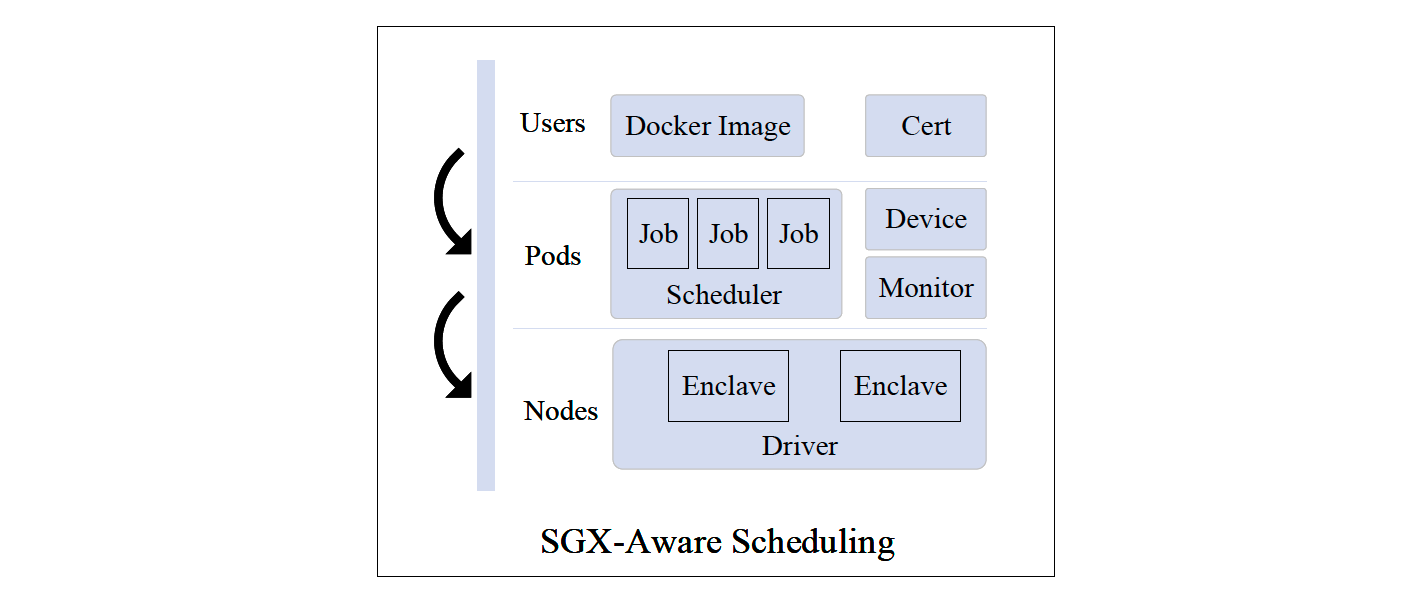
\includegraphics[width=\textwidth]{figures/sgx-aware-sche.png}}
    \caption{SGX可感知的调度系统。}
    \label{sgx_aware_sche}
\end{figure}

Neuchâtel大学的S. Vaucher等人\parencite{vaucher2018sgx}在这个方向上做了进一步的工作,基于Kubernetes实现了SGX可感知的集群管理系统。图是~\ref{sgx_aware_sche}SGX 可感知的集群管理系统的系统架构,该系统主要在四个方面做出了改进:第一,基于Kubernetes 的设备插件机制,实现了SGX 设备的接入。第二,基于节点EPC 实时使用情况实现SGX 可感知的容器调度。第三,基于Kubernetes 的监控模块Heapster 以及时序数据库InfluxQL 实现集群对各节点EPC 使用情况的实时监控。第四,修改Intel 官方的原生SGX 驱动程序,实现EPC 实时使用数据的信息采集以及限制容器使用EPC 的大小,防止因EPC 资源竞争而导致程序性能下降。

\subsection{在机器学习任务中应用SGX技术}
由于SGX EPC大小的限制(可供应用程序使用的仅有不足100MB),在实际生产环境中很难直接应用于大型机器学习模型的训练,多数情况下SGX被用于有隐私需求的模型部署。尽管如此O. Ohrimenko等人\parencite{197247}和R. Kunkel\parencite{kunkel2019tensorscone}等人还是在SGX环境下的机器学习模型训练做了若干尝试。O. Ohrimenko等人在SGX环境下实现了若干传统的机器学习算法如K-means,SVM,decision-tree等,并证实了其性能在一定程度上是可以接受的。

\begin{figure}[h]
    \centerline{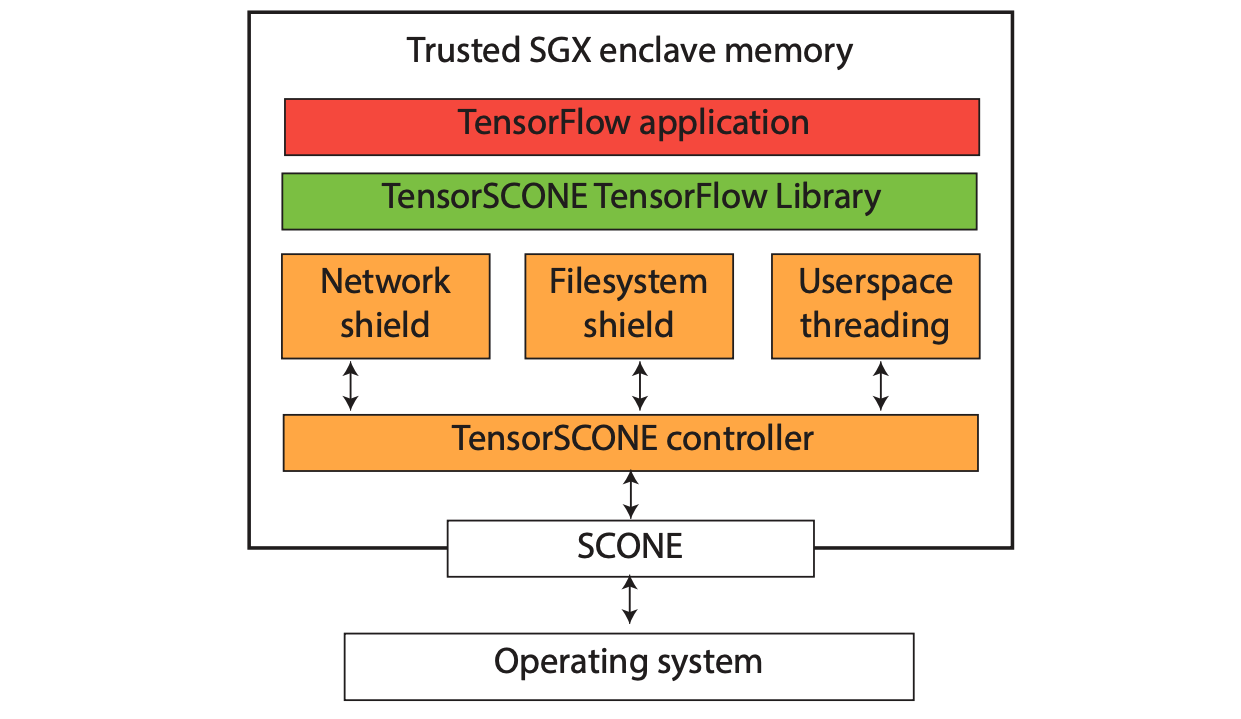
\includegraphics[width=\textwidth]{figures/tensorscone-arch.png}}
    \caption{TensorSCONE架构图。}
    \label{tensorscone_arch}
\end{figure}

R. Kunkel则基于其前序工作SCONE\parencite{arnautov2016scone}实现了支持机器学习任务的安全容器环境TensorSCONE。图~\ref{tensorscone_arch}阐述了TensorSCONE的架构示意图。TensorSCONE基于的SCONE是与Docker完全兼容的,且实现了标准的本地认证和远程认证API。考虑到在EPC受限的环境中应该采用尽可能轻量级的框架,其在应用层框架上其选择了较为轻量的机器学习框架Tensorflow Lite(TF Lite)。其在SCONE容器内部实现了一个定制化的controller,负责重载TF Lite的若干功能,并为上层应用提供统一的接口。在其实验中,其仅测试了ML任务的模型推断,并称利用TensorSCONE框架训练一个Inception模型可能需要数月的时间。

J. Ma在2020年提出了S3ML\parencite{ma2020s3ml},基于服务器端的可信执行环境技术SGX来实现云端机器学习模型部署的安全可信。图~\ref{s3ml_arch}表述了S3ML的架构。S3ML从两个方面来提升云原生共享集群对安全可信应用的支持。首先,S3ML抽象凝练了开发者在使用可信计算环境技术构建应用中所面临的共性需求,将密钥生成、分发、持久化等必备功能实现成独立的安全服务。依赖于该服务,应用开发的效率可以显著提升。其次,在管理可信执行环境设备方面,S3ML提出了一种方法,在给定一个服务SLO的情况下对服务进行离线性能分析,探索服务延时与硬件资源指标的定量定性关系。进一步地,S3ML提出新的系统架构与机制,合理利用SGX特殊硬件资源的实时监控信息,保障在运行着混合负载、存在资源争用的共享集群里依然能够满足服务SLO。

\begin{figure}[h]
    \centerline{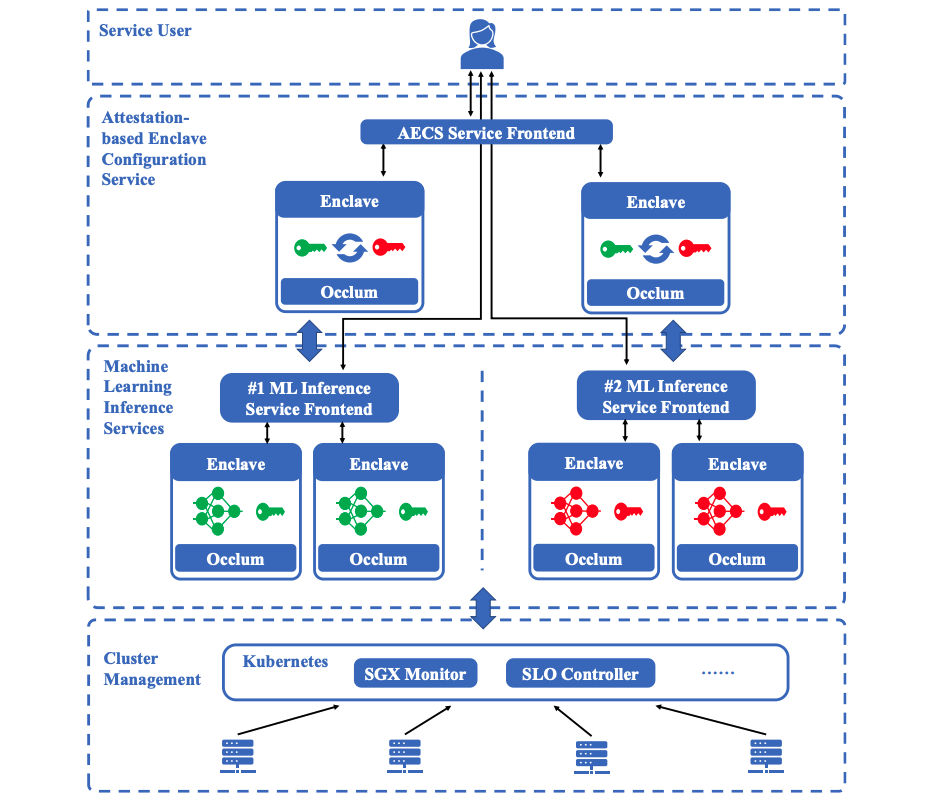
\includegraphics[width=\textwidth]{figures/s3ml-arch.png}}
    \caption{S3ML架构示意图。}
    \label{s3ml_arch}
\end{figure}

\section{小结}
本章介绍了加速型硬件GPU和安全型硬件SGX在云环境中为机器学习带来的新的机遇和挑战。对于GPU的利用,本章从两个角度展开。第一个是集群环境中以单个GPU为最小调度单位的GPU集群调度算法,该类算法一般关注GPU之间的连接和拓扑结构,旨在实现一定的任务放置策略使得任务性能最大化、集群吞吐率最大化。同时,结合优先级分级的方法,使得低优先级的任务可以在机会性资源上运行,可以进一步提升集群的资源利用率。另一个角度是多个ML任务共用同一个GPU。从本质上讲,这也是一种GPU调度的场景,只不过最小调度单位是部分GPU。这种场景下,除了传统的GPU虚拟化手段,近年来越来越多的研究人员尝试在特定的业务场景下(机器学习模型的训练即为一个典型的场景)实现特定的GPU共享机制。SGX是云环境中支持安全计算的硬件。由于其兴起时间较晚,因此在其上运行机器学习负载的研究还处于探索阶段,未能大规模应用于生产环境。事实上,Intel计划在不久的未来随着新架构CPU的发布对SGX技术做同步更新,其所能支持的EPC上限可能会大幅度提升,这无疑会给大规模模型的安全训练和部署带来新的潜在解决方案。未来一段时间内,机器学习任务针对GPU和SGX的研究将持续称为学术界的研究热点。
% vim:ts=4:sw=4
